\documentclass{beamer}

% Recommended beamer themes:
% \usetheme{Madrid}        % Clean and modern
\usetheme{Berlin}        % Simple, with sidebar
% \usetheme{Frankfurt}     % Minimal, with top navigation
% \usetheme{CambridgeUS}   % Classic academic look
% \usetheme{Bergen}        % Elegant, with sidebar
% \usetheme{AnnArbor}      % Colorful, with sidebar
% \usetheme{Darmstadt}     % Professional, with sidebar
% \usetheme{Singapore}     % Clean, with sidebar
% \usetheme{Warsaw}        % Modern, with navigation bar


% 图形与排版支持
\usepackage{graphicx}       % 图形插入支持
\usepackage{adjustbox}      % 高级图片调整
\usepackage{framed}         % 边框环境
\usepackage{amssymb,amsfonts} % 数学符号和字体支持
% \usepackage{amsthm}         % 定理环境支持
\usepackage[dvipsnames]{xcolor} % 颜色支持
\usepackage[most]{tcolorbox} % 彩色盒子环境
\usepackage{tikz}           % 矢量绘图
\usepackage{tikz-cd}        % 交换图绘制
\usepackage[all]{xy}        % 交换图绘制
%%
% \usepackage{enumitem}       % 自定义列表标签
%%

\usepackage[backend=biber,style=alphabetic]{biblatex} % 参考文献管理
\addbibresource{ref.bib}

\usepackage[nameinlink]{cleveref} % 智能引用(自动添加前缀)

% 定理环境定义
\newtheorem{conjecture}{Conjecture}
\newtheorem{question}{Question}
% \newtheorem{definition}{Definition}

% 中文支持
\usepackage[scheme=plain]{ctex} % 中文基础方案
\usepackage{fontspec}      % 字体配置

% Unicode数学字体支持
\usepackage{unicode-math}
\setmainfont{Times New Roman}
\setmathfont{Cambria Math}
\setmathfont{STIX Two Math}[range=cal]
\setmathfont{Libertinus Math}[range=scr]

%一些常用的宏定义
\newcommand{\bbA}{{\mathbb{A}}}
\newcommand{\bba}{{\mathbb{a}}}
\newcommand{\bbB}{{\mathbb{B}}}
\newcommand{\bbb}{{\mathbb{b}}}
\newcommand{\bbC}{{\mathbb{C}}}
\newcommand{\bbc}{{\mathbb{c}}}
\newcommand{\bbD}{{\mathbb{D}}} 
\newcommand{\bbd}{{\mathbb{d}}}
\newcommand{\bbE}{{\mathbb{E}}}
\newcommand{\bbe}{{\mathbb{e}}}
\newcommand{\bbF}{{\mathbb{F}}}
\newcommand{\bbf}{{\mathbb{f}}}
\newcommand{\bbG}{{\mathbb{G}}}
\newcommand{\bbg}{{\mathbb{g}}}
\newcommand{\bbH}{{\mathbb{H}}}
\newcommand{\bbh}{{\mathbb{h}}}
\newcommand{\bbI}{{\mathbb{I}}}
\newcommand{\bbi}{{\mathbb{i}}}
\newcommand{\bbJ}{{\mathbb{J}}}
\newcommand{\bbj}{{\mathbb{j}}}
\newcommand{\bbK}{{\mathbb{K}}}
\newcommand{\bbk}{{\mathbb{k}}}
\newcommand{\bbL}{{\mathbb{L}}}
\newcommand{\bbl}{{\mathbb{l}}}
\newcommand{\bbM}{{\mathbb{M}}}
\newcommand{\bbm}{{\mathbb{m}}}
\newcommand{\bbN}{{\mathbb{N}}}
\newcommand{\bbn}{{\mathbb{n}}}
\newcommand{\bbO}{{\mathbb{O}}}
\newcommand{\bbo}{{\mathbb{o}}}
\newcommand{\bbP}{{\mathbb{P}}}
\newcommand{\bbp}{{\mathbb{p}}}
\newcommand{\bbQ}{{\mathbb{Q}}}
\newcommand{\bbq}{{\mathbb{q}}}
\newcommand{\bbR}{{\mathbb{R}}}
\newcommand{\bbr}{{\mathbb{r}}}
\newcommand{\bbS}{{\mathbb{S}}}
\newcommand{\bbs}{{\mathbb{s}}}
\newcommand{\bbT}{{\mathbb{T}}}
\newcommand{\bbt}{{\mathbb{t}}}
\newcommand{\bbU}{{\mathbb{U}}}
\newcommand{\bbu}{{\mathbb{u}}}
\newcommand{\bbV}{{\mathbb{V}}}
\newcommand{\bbv}{{\mathbb{v}}}
\newcommand{\bbW}{{\mathbb{W}}}
\newcommand{\bbw}{{\mathbb{w}}}
\newcommand{\bbX}{{\mathbb{X}}}
\newcommand{\bbx}{{\mathbb{x}}}
\newcommand{\bbY}{{\mathbb{Y}}}
\newcommand{\bby}{{\mathbb{y}}}
\newcommand{\bbZ}{{\mathbb{Z}}}
\newcommand{\bbz}{{\mathbb{z}}}
\newcommand{\bbone}{{\mathbb{1}}}

\newcommand{\calA}{{\mathcal{A}}}
\newcommand{\cala}{{\mathcal{a}}}
\newcommand{\calB}{{\mathcal{B}}}
\newcommand{\calb}{{\mathcal{b}}}
\newcommand{\calC}{{\mathcal{C}}}
\newcommand{\calc}{{\mathcal{c}}}
\newcommand{\calD}{{\mathcal{D}}}
\newcommand{\cald}{{\mathcal{d}}}
\newcommand{\calE}{{\mathcal{E}}}
\newcommand{\cale}{{\mathcal{e}}}
\newcommand{\calF}{{\mathcal{F}}}
\newcommand{\calf}{{\mathcal{f}}}
\newcommand{\calG}{{\mathcal{G}}}
\newcommand{\calg}{{\mathcal{g}}}
\newcommand{\calH}{{\mathcal{H}}}
\newcommand{\calh}{{\mathcal{h}}}
\newcommand{\calI}{{\mathcal{I}}}
\newcommand{\cali}{{\mathcal{i}}}
\newcommand{\calJ}{{\mathcal{J}}}
\newcommand{\calj}{{\mathcal{j}}}
\newcommand{\calK}{{\mathcal{K}}}
\newcommand{\calk}{{\mathcal{k}}}
\newcommand{\calL}{{\mathcal{L}}}
\newcommand{\call}{{\mathcal{l}}}
\newcommand{\calM}{{\mathcal{M}}}
\newcommand{\calm}{{\mathcal{m}}}
\newcommand{\calN}{{\mathcal{N}}}
\newcommand{\caln}{{\mathcal{n}}}
\newcommand{\calO}{{\mathcal{O}}}
\newcommand{\calo}{{\mathcal{o}}}
\newcommand{\calP}{{\mathcal{P}}}
\newcommand{\calp}{{\mathcal{p}}}
\newcommand{\calQ}{{\mathcal{Q}}}
\newcommand{\calq}{{\mathcal{q}}}
\newcommand{\calR}{{\mathcal{R}}}
\newcommand{\calr}{{\mathcal{r}}}
\newcommand{\calS}{{\mathcal{S}}}
\newcommand{\cals}{{\mathcal{s}}}
\newcommand{\calT}{{\mathcal{T}}}
\newcommand{\calt}{{\mathcal{t}}}
\newcommand{\calU}{{\mathcal{U}}}
\newcommand{\calu}{{\mathcal{u}}}
\newcommand{\calV}{{\mathcal{V}}}
\newcommand{\calv}{{\mathcal{v}}}
\newcommand{\calW}{{\mathcal{W}}}
\newcommand{\calw}{{\mathcal{w}}}
\newcommand{\calX}{{\mathcal{X}}}
\newcommand{\calx}{{\mathcal{x}}}
\newcommand{\calY}{{\mathcal{Y}}}
\newcommand{\caly}{{\mathcal{y}}}
\newcommand{\calZ}{{\mathcal{Z}}}
\newcommand{\calz}{{\mathcal{z}}}

\newcommand{\frakA}{{\mathfrak{A}}}
\newcommand{\fraka}{{\mathfrak{a}}}
\newcommand{\frakB}{{\mathfrak{B}}}
\newcommand{\frakb}{{\mathfrak{b}}}
\newcommand{\frakC}{{\mathfrak{C}}}
\newcommand{\frakc}{{\mathfrak{c}}}
\newcommand{\frakD}{{\mathfrak{D}}}
\newcommand{\frakd}{{\mathfrak{d}}}
\newcommand{\frakE}{{\mathfrak{E}}}
\newcommand{\frake}{{\mathfrak{e}}}
\newcommand{\frakF}{{\mathfrak{F}}}
\newcommand{\frakf}{{\mathfrak{f}}}
\newcommand{\frakG}{{\mathfrak{G}}}
\newcommand{\frakg}{{\mathfrak{g}}}
\newcommand{\frakH}{{\mathfrak{H}}}
\newcommand{\frakh}{{\mathfrak{h}}}
\newcommand{\frakI}{{\mathfrak{I}}}
\newcommand{\fraki}{{\mathfrak{i}}}
\newcommand{\frakJ}{{\mathfrak{J}}}
\newcommand{\frakj}{{\mathfrak{j}}}
\newcommand{\frakK}{{\mathfrak{K}}}
\newcommand{\frakk}{{\mathfrak{k}}}
\newcommand{\frakL}{{\mathfrak{L}}}
\newcommand{\frakl}{{\mathfrak{l}}}
\newcommand{\frakM}{{\mathfrak{M}}}
\newcommand{\frakm}{{\mathfrak{m}}}
\newcommand{\frakN}{{\mathfrak{N}}}
\newcommand{\frakn}{{\mathfrak{n}}}
\newcommand{\frakO}{{\mathfrak{O}}}
\newcommand{\frako}{{\mathfrak{o}}}
\newcommand{\frakP}{{\mathfrak{P}}}
\newcommand{\frakp}{{\mathfrak{p}}}
\newcommand{\frakQ}{{\mathfrak{Q}}}
\newcommand{\frakq}{{\mathfrak{q}}}
\newcommand{\frakR}{{\mathfrak{R}}}
\newcommand{\frakr}{{\mathfrak{r}}}
\newcommand{\frakS}{{\mathfrak{S}}}
\newcommand{\fraks}{{\mathfrak{s}}}
\newcommand{\frakT}{{\mathfrak{T}}}
\newcommand{\frakt}{{\mathfrak{t}}}
\newcommand{\frakU}{{\mathfrak{U}}}
\newcommand{\fraku}{{\mathfrak{u}}}
\newcommand{\frakV}{{\mathfrak{V}}}
\newcommand{\frakv}{{\mathfrak{v}}}
\newcommand{\frakW}{{\mathfrak{W}}}
\newcommand{\frakw}{{\mathfrak{w}}}
\newcommand{\frakX}{{\mathfrak{X}}}
\newcommand{\frakx}{{\mathfrak{x}}}
\newcommand{\frakY}{{\mathfrak{Y}}}
\newcommand{\fraky}{{\mathfrak{y}}}
\newcommand{\frakZ}{{\mathfrak{Z}}}
\newcommand{\frakz}{{\mathfrak{z}}}

\newcommand{\rmA}{{\mathrm{A}}}
\newcommand{\rma}{{\mathrm{a}}}
\newcommand{\rmB}{{\mathrm{B}}}
\newcommand{\rmb}{{\mathrm{b}}}
\newcommand{\rmC}{{\mathrm{C}}}
\newcommand{\rmc}{{\mathrm{c}}}
\newcommand{\rmD}{{\mathrm{D}}}
\newcommand{\rmd}{{\mathrm{d}}}
\newcommand{\rmE}{{\mathrm{E}}}
\newcommand{\rme}{{\mathrm{e}}}
\newcommand{\rmF}{{\mathrm{F}}}
\newcommand{\rmf}{{\mathrm{f}}}
\newcommand{\rmG}{{\mathrm{G}}}
\newcommand{\rmg}{{\mathrm{g}}}
\newcommand{\rmH}{{\mathrm{H}}}
\newcommand{\rmh}{{\mathrm{h}}}
\newcommand{\rmI}{{\mathrm{I}}}
\newcommand{\rmi}{{\mathrm{i}}}
\newcommand{\rmJ}{{\mathrm{J}}}
\newcommand{\rmj}{{\mathrm{j}}}
\newcommand{\rmK}{{\mathrm{K}}}
\newcommand{\rmk}{{\mathrm{k}}}
\newcommand{\rmL}{{\mathrm{L}}}
\newcommand{\rml}{{\mathrm{l}}}
\newcommand{\rmM}{{\mathrm{M}}}
\newcommand{\rmm}{{\mathrm{m}}}
\newcommand{\rmN}{{\mathrm{N}}}
\newcommand{\rmn}{{\mathrm{n}}}
\newcommand{\rmO}{{\mathrm{O}}}
\newcommand{\rmo}{{\mathrm{o}}}
\newcommand{\rmP}{{\mathrm{P}}}
\newcommand{\rmp}{{\mathrm{p}}}
\newcommand{\rmQ}{{\mathrm{Q}}}
\newcommand{\rmq}{{\mathrm{q}}}
\newcommand{\rmR}{{\mathrm{R}}}
\newcommand{\rmr}{{\mathrm{r}}}
\newcommand{\rmS}{{\mathrm{S}}}
\newcommand{\rms}{{\mathrm{s}}}
\newcommand{\rmT}{{\mathrm{T}}}
\newcommand{\rmt}{{\mathrm{t}}}
\newcommand{\rmU}{{\mathrm{U}}}
\newcommand{\rmu}{{\mathrm{u}}}
\newcommand{\rmV}{{\mathrm{V}}}
\newcommand{\rmv}{{\mathrm{v}}}
\newcommand{\rmW}{{\mathrm{W}}}
\newcommand{\rmw}{{\mathrm{w}}}
\newcommand{\rmX}{{\mathrm{X}}}
\newcommand{\rmx}{{\mathrm{x}}}
\newcommand{\rmY}{{\mathrm{Y}}}
\newcommand{\rmy}{{\mathrm{y}}}
\newcommand{\rmZ}{{\mathrm{Z}}}

\newcommand{\bfA}{{\mathbf{A}}}
\newcommand{\bfa}{{\mathbf{a}}}
\newcommand{\bfB}{{\mathbf{B}}}
\newcommand{\bfb}{{\mathbf{b}}}
\newcommand{\bfC}{{\mathbf{C}}}
\newcommand{\bfc}{{\mathbf{c}}}
\newcommand{\bfD}{{\mathbf{D}}}
\newcommand{\bfd}{{\mathbf{d}}}
\newcommand{\bfE}{{\mathbf{E}}}
\newcommand{\bfe}{{\mathbf{e}}}
\newcommand{\bfF}{{\mathbf{F}}}
\newcommand{\bff}{{\mathbf{f}}}
\newcommand{\bfG}{{\mathbf{G}}}
\newcommand{\bfg}{{\mathbf{g}}}
\newcommand{\bfH}{{\mathbf{H}}}
\newcommand{\bfh}{{\mathbf{h}}}
\newcommand{\bfI}{{\mathbf{I}}}
\newcommand{\bfi}{{\mathbf{i}}}
\newcommand{\bfJ}{{\mathbf{J}}}
\newcommand{\bfj}{{\mathbf{j}}}
\newcommand{\bfK}{{\mathbf{K}}}
\newcommand{\bfk}{{\mathbf{k}}}
\newcommand{\bfL}{{\mathbf{L}}}
\newcommand{\bfl}{{\mathbf{l}}}
\newcommand{\bfM}{{\mathbf{M}}}
\newcommand{\bfm}{{\mathbf{m}}}
\newcommand{\bfN}{{\mathbf{N}}}
\newcommand{\bfn}{{\mathbf{n}}}
\newcommand{\bfO}{{\mathbf{O}}}
\newcommand{\bfo}{{\mathbf{o}}}
\newcommand{\bfP}{{\mathbf{P}}}
\newcommand{\bfp}{{\mathbf{p}}}
\newcommand{\bfQ}{{\mathbf{Q}}}
\newcommand{\bfq}{{\mathbf{q}}}
\newcommand{\bfR}{{\mathbf{R}}}
\newcommand{\bfr}{{\mathbf{r}}}
\newcommand{\bfS}{{\mathbf{S}}}
\newcommand{\bfs}{{\mathbf{s}}}
\newcommand{\bfT}{{\mathbf{T}}}
\newcommand{\bft}{{\mathbf{t}}}
\newcommand{\bfU}{{\mathbf{U}}}
\newcommand{\bfu}{{\mathbf{u}}}
\newcommand{\bfV}{{\mathbf{V}}}
\newcommand{\bfv}{{\mathbf{v}}}
\newcommand{\bfW}{{\mathbf{W}}}
\newcommand{\bfw}{{\mathbf{w}}}
\newcommand{\bfX}{{\mathbf{X}}}
\newcommand{\bfx}{{\mathbf{x}}}
\newcommand{\bfY}{{\mathbf{Y}}}
\newcommand{\bfy}{{\mathbf{y}}}
\newcommand{\bfZ}{{\mathbf{Z}}}
\newcommand{\bfz}{{\mathbf{z}}}

\newcommand{\sfA}{{\mathsf{A}}}
\newcommand{\sfa}{{\mathsf{a}}}
\newcommand{\sfB}{{\mathsf{B}}}
\newcommand{\sfb}{{\mathsf{b}}}
\newcommand{\sfC}{{\mathsf{C}}}
\newcommand{\sfc}{{\mathsf{c}}}
\newcommand{\sfD}{{\mathsf{D}}}
\newcommand{\sfd}{{\mathsf{d}}}
\newcommand{\sfE}{{\mathsf{E}}}
\newcommand{\sfe}{{\mathsf{e}}}
\newcommand{\sfF}{{\mathsf{F}}}
\newcommand{\sff}{{\mathsf{f}}}
\newcommand{\sfG}{{\mathsf{G}}}
\newcommand{\sfg}{{\mathsf{g}}}
\newcommand{\sfH}{{\mathsf{H}}}
\newcommand{\sfh}{{\mathsf{h}}}
\newcommand{\sfI}{{\mathsf{I}}}
\newcommand{\sfi}{{\mathsf{i}}}
\newcommand{\sfJ}{{\mathsf{J}}}
\newcommand{\sfj}{{\mathsf{j}}}
\newcommand{\sfK}{{\mathsf{K}}}
\newcommand{\sfk}{{\mathsf{k}}}
\newcommand{\sfL}{{\mathsf{L}}}
\newcommand{\sfl}{{\mathsf{l}}}
\newcommand{\sfM}{{\mathsf{M}}}
\newcommand{\sfm}{{\mathsf{m}}}
\newcommand{\sfN}{{\mathsf{N}}}
\newcommand{\sfn}{{\mathsf{n}}}
\newcommand{\sfO}{{\mathsf{O}}}
\newcommand{\sfo}{{\mathsf{o}}}
\newcommand{\sfP}{{\mathsf{P}}}
\newcommand{\sfp}{{\mathsf{p}}}
\newcommand{\sfQ}{{\mathsf{Q}}}
\newcommand{\sfq}{{\mathsf{q}}}
\newcommand{\sfR}{{\mathsf{R}}}
\newcommand{\sfr}{{\mathsf{r}}}
\newcommand{\sfS}{{\mathsf{S}}}
\newcommand{\sfs}{{\mathsf{s}}}
\newcommand{\sfT}{{\mathsf{T}}}
\newcommand{\sft}{{\mathsf{t}}}
\newcommand{\sfU}{{\mathsf{U}}}
\newcommand{\sfu}{{\mathsf{u}}}
\newcommand{\sfV}{{\mathsf{V}}}
\newcommand{\sfv}{{\mathsf{v}}}
\newcommand{\sfW}{{\mathsf{W}}}
\newcommand{\sfw}{{\mathsf{w}}}
\newcommand{\sfX}{{\mathsf{X}}}
\newcommand{\sfx}{{\mathsf{x}}}
\newcommand{\sfY}{{\mathsf{Y}}}
\newcommand{\sfy}{{\mathsf{y}}}
\newcommand{\sfZ}{{\mathsf{Z}}}
\newcommand{\sfz}{{\mathsf{z}}}


\newcommand{\kk}{{\mathbf{k}}}
\newcommand{\kkk}{{\mathbb{k}}}
\newcommand{\KK}{{\mathbf{K}}}
\newcommand{\KKK}{{\mathbb{K}}}
\newcommand{\rkk}{{\kappa}} % residue field
\newcommand{\fkk}{{\mathscr{K}}} % fraction field

\renewcommand{\d}{{\mathrm{d}}}
\renewcommand{\i}{{\mathrm{i}}}
\renewcommand{\P}{\partial}


\newcommand{\Set}{\mathbf{Set}}
\newcommand{\Var}{\mathbf{Var}}
\newcommand{\Sch}{\mathbf{Sch}}
\newcommand{\Alg}{\mathbf{Alg}}
\newcommand{\Ring}{\mathbf{Ring}}
\newcommand{\Mod}{\mathbf{Mod}}
\newcommand{\TopMod}{\mathbf{TopMod}}
\newcommand{\Grp}{\mathbf{Grp}}
\newcommand{\Ab}{\mathbf{Ab}}
\newcommand{\Top}{\mathbf{Top}}
\newcommand{\Cat}{\mathbf{Cat}}
\newcommand{\AlgSp}{\mathbf{AlgSp}}
\newcommand{\Obj}{\operatorname{Obj}}


\newcommand{\ten}{\otimes}
\newcommand{\ratmap}{\dasharrow}
\newcommand{\injmap}{\hookrightarrow}
\newcommand{\surjmap}{\twoheadrightarrow}

\newcommand{\id}{{\operatorname{id}}}

\newcommand{\Frac}{\operatorname{Frac}}
\newcommand{\Der}{\operatorname{Der}}
\newcommand{\Spec}{\operatorname{Spec}}
\newcommand{\spec}{\operatorname{Spec}}
\newcommand{\mSpec}{\operatorname{mSpec}}
\newcommand{\depth}{\operatorname{depth}}
\newcommand{\idealht}{\operatorname{ht}}
\newcommand{\codim}{\operatorname{codim}}
\newcommand{\Supp}{\operatorname{Supp}}
\newcommand{\trdeg}{\operatorname{trdeg}}
\newcommand{\Ass}{\operatorname{Ass}}
\newcommand{\Ann}{\operatorname{Ann}}
\newcommand{\Ext}{\operatorname{Ext}}
\newcommand{\Tor}{\operatorname{Tor}}
\newcommand{\Hom}{\operatorname{Hom}}
\newcommand{\Eq}{\operatorname{Eq}}
\newcommand{\End}{\operatorname{End}}
\newcommand{\Mor}{\operatorname{Mor}}
\newcommand{\Mult}{\operatorname{Mult}}
\renewcommand{\Im}{\operatorname{Im}}
\newcommand{\Ker}{\operatorname{Ker}}
\newcommand{\rank}{\operatorname{rank}}
\newcommand{\cohdim}{\operatorname{coh.dim}}
\newcommand{\hldim}{\operatorname{hl.dim}}
\newcommand{\projdim}{\operatorname{proj.dim}}
\newcommand{\injdim}{\operatorname{inj.dim}}
\newcommand{\rad}{\operatorname{rad}}
\newcommand{\nil}{\operatorname{nil}}
\newcommand{\characteristic}{\operatorname{char}}
\newcommand{\Pic}{\operatorname{Pic}}
\newcommand{\NS}{\operatorname{NS}}
\newcommand{\Exc}{\operatorname{Exc}}
\newcommand{\Sing}{\operatorname{Sing}}
\newcommand{\Reg}{\operatorname{Reg}}
\newcommand{\Tr}{\operatorname{Tr}}
\newcommand{\Psef}{\operatorname{Psef}}
\newcommand{\Nef}{\operatorname{Nef}}
\newcommand{\Amp}{\operatorname{Amp}}
\newcommand{\Bigcone}{\operatorname{Big}}
\newcommand{\Frob}{\operatorname{Frob}}
\newcommand{\Bs}{\operatorname{Bs}}
\newcommand{\Stab}{\operatorname{Stab}}
\newcommand{\Sp}{\operatorname{Sp}}


\newcommand{\calHom}{{\mathcal{H\!o\!m}}}
\newcommand{\calExt}{{\mathcal{Ext}}}
\newcommand{\calProj}{{\mathcal{P\!r\!o\!j}}}
\newcommand{\calSpec}{{\mathcal{S\!p\!e\!c}}}


\newcommand{\mat}[4]{\left[ \begin{array}{cc}#1 &#2 \\ #3 &#4\end{array}\right]}
\newcommand{\threemat}[9]{\left[ \begin{array}{ccc}
  #1 & #2 & #3 \\
  #4 & #5 & #6 \\
  #7 & #8 & #9
\end{array}\right]}
\newcommand{\genmat}[9]{\left( \begin{array}{cccc}
  #1 & #2 & \cdots & #3 \\
  #4 & #5 & \cdots & #6 \\  
  \ldots & \ldots & \ddots & \ldots \\
  #7 & #8 & \cdots & #9
\end{array}\right)}





\newcommand{\contradiction}{
    \raisebox{-0.6ex}{\makebox[2.4ex][c]{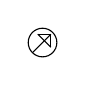
\begin{tikzpicture}
        \draw (0,0) circle (1.2ex);
        \draw (0.7 ex, 0.7 ex) -- (-0.4 ex, 0.7 ex);
        \draw (-0.4 ex, 0.7 ex) -- (0.7 ex, -0.4 ex);
        \draw (0.7 ex, -0.4 ex) -- (0.7 ex, 0.7 ex);
        \draw (0.7 ex, 0.7 ex) -- (-0.848 ex, -0.848 ex);
    \end{tikzpicture}}}
    \ \ 
}

% legendre符号
\makeatletter
\def\legendre@dash#1#2{\hb@xt@#1{%
  \kern-#2\p@
  \cleaders\hbox{\kern.5\p@
    \vrule\@height.2\p@\@depth.2\p@\@width\p@
    \kern.5\p@}\hfil
  \kern-#2\p@
  }}
\def\@legendre#1#2#3#4#5{\mathopen{}\left(
  \sbox\z@{$\genfrac{}{}{0pt}{#1}{#3#4}{#3#5}$}%
  \dimen@=\wd\z@
  \kern-\p@\vcenter{\box0}\kern-\dimen@\vcenter{\legendre@dash\dimen@{#2}}\kern-\p@
  \right)\mathclose{}}
\newcommand\legendre[2]{\mathchoice
  {\@legendre{0}{1}{}{#1}{#2}}
  {\@legendre{1}{.5}{\vphantom{1}}{#1}{#2}}
  {\@legendre{2}{0}{\vphantom{1}}{#1}{#2}}
  {\@legendre{3}{0}{\vphantom{1}}{#1}{#2}}
}
\def\dlegendre{\@legendre{0}{1}{}}
\def\tlegendre{\@legendre{1}{0.5}{\vphantom{1}}}
\makeatother

% \usepackage{mathabx,epsfig}
\def\acts{\ \rotatebox[origin=c]{-90}{$\circlearrowright$}\ }
\def\racts{\ \rotatebox[origin=c]{90}{$\circlearrowleft$}\ }
\def\dacts{\ \rotatebox[origin=c]{0}{$\circlearrowright$}\ }
\def\uacts{\ \rotatebox[origin=c]{180}{$\circlearrowright$}\ }

\title{Dynamical Iitaka Theory on Fano Contractions}
\author{Tianle Yang, \\ joint work with Sheng Meng and Long Wang}
\date{2025.08.20}

\begin{document}

\begin{frame}
    \titlepage
\end{frame}

\begin{frame}{Outline}
    \tableofcontents
\end{frame}

\section{Kawaguchi-Silverman Conjecture}
\begin{frame}{Algebraic Dynamics}
    We work over \(\overline{\bbQ}\).
    The fundamental objects in algebraic dynamics are \((X,f)\), where \(X\) is a projective variety and \(f:X \dashrightarrow X\) is a dominant rational self-map.
    Here we focus on the case \(f\) is a surjective endomorphism.
    
\end{frame}

\begin{frame}{Dynamical degree}

    \begin{definition}[First dynamical degree]\label{def: delta_f}
        Consider a projective variety \(X\) and a surjective endomorphism $f:X\to X$.
        The \textit{first dynamical degree} \(\delta_f\) of \(f\) is defined to be the following limit
        \[
        \delta_f := \lim_{n\to\infty}((f^n)^*H\cdot H^{\dim X-1})^{1/n}\in\mathbb{R}_{\geq 1},
        \]
        where $H$ is an ample Cartier divisor.
    \end{definition}

    \pause

    It is known that the limit always exists and is independent of the choice of $H$  (see \cite{DS04,DS05}; cf.~\cite{Dan20}). 
    
    \pause

    It is also known that the first dynamical degree \(\delta_f\) coincides with the spectral radius of the induced linear operation \(f^*|_{\textup{N}^1(X)}\).

\end{frame}

\begin{frame}{Height function}

    Recall that for every line bundle \(\calL\), there is a height function \(h_\calL\colon X(\overline{\bbQ})\to\mathbb{R}\) associated to \(\calL\), 
    which measures the arithmetic complexity of \(\overline{\bbQ}\)-points and is unique up to a bounded function.
    
    \pause

    For example, if \(X = \bbP^n\), \(\calL = \calO_{\bbP^n}(1)\) and \(x = [x_0:\cdots:x_n]\in X(\bbQ)\) with \(x_i\in \bbZ\) and \(\gcd(x_0,\ldots,x_n)=1\), then
    \[ h_{\calO_{\bbP^n}(1)}(x) = \max\{|x_0|,\ldots,|x_n|\} \]
    is the standard height function on \(\bbP^n\).

    \pause

    In general, if \(H\) is a very ample Cartier divisor on \(X\) associated to a closed immersion \(\varphi: X\hookrightarrow \bbP^N\), one can define the Weil height function \(h_H\) by
    \[ h_H(x) = h_{\calO_{\bbP^N}(1)}(\varphi(x)). \]

\end{frame}
\begin{frame}{Arithmetic degree}

    \begin{definition}[Arithmetic degree]\label{def: alpha_f}
        Let \(h_H\geq 1\) be a Weil height function associated with an ample Cartier divisor \(H\).
        Then for every \(x\in X(\overline{\bbQ})\), we define the \emph{arithmetic degree of \(f\) at \(x\)} by
        \[
        \alpha_f(x)=\lim_{n\to\infty}h_H(f^n(x))^{1/n}\in\mathbb{R}_{\geq 1}.
        \]
    \end{definition}

    \pause

    Due to Kawaguchi-Silverman \cite{KS16a}, the limit always exists and is also independent of the choice of the ample Cartier divisor and the Weil height function. 
    
    \pause

    Moreover, \(\alpha_f(x)\) is equal to norm of an eigenvalue of \(f^*|_{\rmN^1(X)_\bbC}\).
    In particular, \(\alpha_f(x) \leq \delta_f\).

    % \pause

    % So, there is a natural question that when \(\alpha_f(x) = \delta_f\) holds for a point \(x\in X(\overline{\bbQ})\).
\end{frame}

\begin{frame}{Kawaguchi-Silverman Conjecture}

    \begin{conjecture}[{Kawaguchi-Silverman Conjecture $=$ KSC}]\label{conj: ksc} 
        Let $f : X \to X$ be a surjective endomorphism of a projective variety $X$ defined over $\overline{\mathbb{Q}}$. 
        Let $x \in X(\overline{\mathbb{Q}})$, and suppose that the (forward) orbit $O_f(x) = \{f^n(x)\, |\, n\ge 0\}$  is Zariski dense in $X$.
        Then the arithmetic degree at $x$ is equal to the dynamical degree of $f$, i.e.,
        $\alpha_f(x) = \delta_f$.
    \end{conjecture} 

    \pause

    \begin{itemize}
        \item KSC is known for abelian varieties (\cite{KS16b},\cite{Sil17}) or \(f\) is polarized (\cite{KS16b}).
        \pause
        \item Suppose that there is an equivariant fibration \(\pi:(X,f) \ratmap (Y,g)\) such that \(\delta_f = \delta_g\). 
            If KSC holds for \((Y,g)\), then KSC holds for \((X,f)\).
    \end{itemize}

\end{frame}


\section{Main Results}
\begin{frame}
    \frametitle{Main Results}

    \begin{theorem}\label{mainthm: abelian}
        Let $f$ be a surjective endomorphism of a smooth projective variety $X$ admitting an extremal Fano contraction $\pi:X\to Y$ to an abelian variety $Y$ of positive dimension.
        Suppose $f$ admits a Zariski dense orbit and $\delta_f>\delta_{f|_Y}$.
        Then the following hold.
        \begin{enumerate}
            \item The ramification divisor satisfies $f^*R_f\equiv \delta_f R_f$.
            \item There exists an $f$-equivariant dominant rational map $\varphi:X\dashrightarrow Z$, 
            which is the $f$-Iitaka fibration of $R_f$, 
            such that $0<\dim Z<\dim X$ and $f|_Z$ is $\delta_f$-polarized.
        \end{enumerate}
    \end{theorem}

\end{frame}

\begin{frame}
    \frametitle{Main Results}

    \begin{theorem}\label{mainthm: rho1}
        Let $f$ be a surjective endomorphism of a smooth projective variety $X$ admitting an $f$-equivariant {\bf smooth} extremal Fano contraction $\pi:X\to Y$ with $\rho(Y)=1$.
        Suppose $\delta_f>\delta_{f|_Y}=1$.
        Then the following hold.
        \begin{enumerate}
            \item The ramification divisor satisfies $f^*R_f\equiv \delta_f R_f$.
            \item There exists an $f$-equivariant dominant rational map $\varphi:X\dashrightarrow Z$, 
            which is the $f$-Iitaka fibration of $R_f$, 
            such that $0<\dim Z<\dim X$ and $f|_Z$ is $\delta_f$-polarized.
        \end{enumerate}
    \end{theorem}

\end{frame}

\begin{frame}
    \frametitle{Main Results}

    \begin{corollary}\label{maincor: abelian}
        KSC holds for any smooth projective variety $X$ admitting an extremal Fano contraction to an abelian variety. 
    \end{corollary}


    \begin{corollary}\label{maincor: pn}
        KSC holds for any $\mathbb{P}^n$-bundle over either a $Q$-abelian variety or a smooth projective variety of Picard number one. 
    \end{corollary}

\end{frame}



\section{Dynamical Iitaka Theory}

\begin{frame}{Dynamical Iitaka fibration}
    
    \begin{theorem}[{\cite[Theorem 4.6]{MZ23b}}]
        Let $f$ be a surjective endomorphism of a normal projective variety $X$.
        Let $D$ be a $\bbQ$-Cartier divisor with $\kappa_f(X,D)\ge 0$.
        Then there is an $f$-equivariant dominant rational map $\phi_{f,D}:X\dashrightarrow Y$ to a normal projective variety $Y$
        (with $f|_Y$ a surjective endomorphism too)
        satisfying the following conditions.
        \begin{enumerate}
            \item $\dim Y=\kappa_f(X,D)$.
            \item Let $\Gamma$ be the graph of $\phi_{f,D}$. Then the induced projection $\Gamma\to Y$ is equi-dimensional.
            \item $\phi_{f,D}$ is birational to the Iitaka fibration of any $D'\in V_f(D)$ with $\kappa(X,D')=\kappa_f(X,D)$. 
        \end{enumerate}
    \end{theorem}

\end{frame}

\begin{frame}{Dynamical Iitaka dimension}

    \begin{definition}[Dynamical Iitaka dimension]
        Let $f$ be a surjective endomorphism of a normal projective variety $X$ and $D$ a $\bbQ$-Cartier divisor.
        Denote by $V_f(D)$ the subspace of $\Pic_{\bbQ}(X)$ spanned by $D_i:=(f^*)^i(D)$ with $i\in\bbZ$.
        Note that $V_f(D)$ is finite dimensional (cf.~\cite[Proposition 3.7]{MZ22}).
        We define the {\it dynamical $f$-Iitaka dimension} of $D$ as 
        $$\kappa_f(X,D):=\max\{\kappa(X,D')\,|\,D'\in V_f(D)\}.$$
        % If $D_0,\cdots, D_n$ are effective and span $V_f(D)$, 
        % then 
        % \[ \kappa_f(X,D)=\kappa(X, \sum\limits_{i=0}^n D_i). \]
    \end{definition}

    \pause

    Note that by ramification formula, we have \(R_{f^s} = \sum_{i=0}^{s-1} (f^i)^* R_f\) and hence \(\kappa_f(X,R_f) = \kappa(X,R_{f^s})\) for  \(s\gg 1\).

\end{frame}

\begin{frame}{Dynamical Iitaka Program for ramification divisor}

    We consider three situations of $\kappa_f(X,R_f)$ and briefly introduce how the dynamical Iitaka theory works.
    
    \pause

    \begin{itemize}
        \item $\kappa_f(X,R_f)=0$. 
            Then $f^{-1}(\Supp R_f)=\Supp R_f$ and the restriction $$f|_{X\backslash \Supp R_f}\colon X\backslash \Supp R_f\to X\backslash \Supp R_f$$ is (quasi-)\'etale.
        
        \pause
        
        \item $0<\kappa_f(X,R_f)<\dim X$.
            We then have an $f$-equivariant dominant rational map
            $$\varphi_{f,R_f}\colon X\dashrightarrow Y$$
            with $0<\dim Y=\kappa_f(X,R_f)<\dim X$.

        \pause

        \item $\kappa_f(X,R_f)=\dim X$. 
            In this case, $R_{f^s}$ is big when $s\gg 1$.
    \end{itemize}

\end{frame}

\begin{frame}{Dynamical Iitaka Program for ramification divisor}

    \begin{question}\label{que: main1}
        Let $f\colon X\to X$ be a surjective endomorphism of a smooth projective variety with $\varphi_{f,R_f}\colon X\dashrightarrow Y$ the induced dynamical Iitaka fibration.
        Suppose $\kappa_f(X, R_f)>0$. 
        When does the equality of first dynamical degrees $\delta_f=\delta_{f|_Y}$ hold and whether $f$ splits into $f|_Y$ and a quasi-\'etale endomorphism?
    \end{question}

    \pause

    \begin{question}[{\cite[Question 6.9]{MZ23b}}]\label{que: main2}
        Let $f\colon X\to X$ be a surjective endomorphism of a smooth projective variety.
        Suppose $R_f$ is big. Is $f$ int-amplified?
    \end{question}

\end{frame}


\begin{frame}{Dynamical Iitaka fibration}

    A special case of the $f$-Iitaka fibration has been studied in \cite[Theorem 7.8]{MZ22}.
    
    \begin{theorem}[{\cite[Theorem 4.8]{MZ23b}}]
        Let $f:X\to X$ be a surjective endomorphism of a projective variety $X$.
        Let $D$ be a $\bbQ$-Cartier divisor such that $f^*D\equiv qD$ for some $q>1$ and $\kappa(X,D)>0$.
        Let $\phi_{f,D}:X\dashrightarrow Y$ be the $f$-Iitaka fibration of $D$.
        Then $f|_Y$ is $q$-polarized.
    \end{theorem}

    \pause

    By the dynamical Iitaka fibration, we hope to show that \(f^*R_f\equiv \delta_f R_f\) and \(0<\kappa_f(X,R_f)<\dim X\) under the assumption of main theorems.
\end{frame}

% \begin{frame}
%     \frametitle{Setup}

%         In follows, we focus on proof of the main theorem about Fano contractions to abelian varieties.


%         \pause

%         We consider the following setup:
%         \begin{itemize}
%             \item \(f \acts X \xrightarrow{\pi} Y \racts g\) an equivariant dynamics;
%             \item \(X\) is smooth and \(Y\) is an abelian variety;
%             \item \(\dim X = n, \dim Y = m, d = n-m\);
%             \item \(\rho(X) = \rho(Y) + 1\);
%             \item general fiber of \(\pi\) is Fano;
%             \item \(\delta_f > \delta_{f|_Y}\).
%         \end{itemize}

% \end{frame}

\section{Decomposition of cones}
\begin{frame}{Decomposition of cones}

    \only<1>{First we show that \(f^*R_f\equiv \delta_f R_f\).
    It follows from the following decomposition of the cone.}
    
    \pause

    \begin{theorem}[Cone Decomposition]\label{thm: cone}
        % Let $f$ be a surjective endomorphism of a normal projective variety $X$.
        Let $\pi:X\to Y$ be an $f$-equivariant surjective morphism to a $\bbQ$-factorial normal projective variety $Y$ with $\rho(X)=\rho(Y)+1$ and $\delta_f>\delta_{f|_Y}$.
        Suppose further either one of the following two assumptions holds.
        \begin{enumerate}
            \item $\Nef(Y)=\Psef(Y)$.
            \item $X$ and $Y$ are smooth and $\pi$ is equi-dimensional.
        \end{enumerate}  
        Then we have the decompositions: 
        $$
        \begin{aligned}
            \Nef(X) = \pi^{\ast}\Nef(Y) \oplus \mathbb{R}_{\geq 0} D, \quad
            \Psef(X) = \pi^{\ast}\Psef(Y) \oplus \mathbb{R}_{\geq 0} D,
        \end{aligned}
        $$
        for some nef and $\pi$-ample Cartier divisor $D$ with $f^*D\equiv \delta_f D$.
    \end{theorem}

\end{frame}

\begin{frame}
    \frametitle{Sketch of proof of the decomposition of cones}

    \begin{itemize}
        \item By the Perron-Frobenius Theorem, there is a nef and $\pi$-ample Cartier divisor $D$ such that \(f^*D\equiv \delta_f D\).
            We show that the numerical dimension \(\nu(X,D) = \dim X - \dim Y\).
            Since it is \(\pi\)-ample, we have \(\nu(X,D) \geq \dim X - \dim Y\).

            If \(D^{\dim X - \dim Y + 1} \not\equiv_w 0\), then \(\pi_* D^{\dim X - \dim Y + 1}\) will be a \(\delta_f\) eigenvector of \(f^*|_{\rmN^1(Y)}\) by relative dynamical degree formula.
            This implies \(\delta_f = \delta_{f|_Y}\), contradicting the assumption.

            \pause

        \item Under the assumption that \(\Nef(Y)=\Psef(Y)\).
            Note that $\pi^*\Nef(Y)+\mathbb{R}_{\ge 0} D$ is a closed subcone of $\Nef(X)$ and it also spans $\rmN^1(X)$.
            Then it suffices to show $D+\pi^*B$ is not big for any nef and non-ample $\bbR$-Cartier divisor $B$ on $Y$.
            Note that $(D+\pi^*B)^{\dim X}=0$ because $D^i\equiv_w0$ for any $i>\dim X-\dim Y$ and $(\pi^*B)^j\equiv_w 0$ for any $j\ge \dim Y$.
    \end{itemize}
\end{frame}

\begin{frame}
    \frametitle{Proof of the decomposition of cones}

    \begin{itemize}
        \item Under the assumption that $X$ and $Y$ are smooth and $\pi$ is equi-dimensional.
            
            Let $B \in \Psef(X)$ and write $B = \pi^*B_Y + aD$.
            Let $C$ be a nef $1$-cycle on \(Y\).
            Note that $\pi^*C$ is a nef $(d+1)$-cycle on \(X\) by the projection formula.
            Then $B\cdot D^d\cdot \pi^*C\ge 0$.
            So we have 
            \begin{align*}
                \pi_*(B\cdot D^d\cdot \pi^*C ) &= \pi_*(\pi^*(B_Y\cdot C) \cdot D^d) + \pi_*(\pi^*C \cdot D^{d+1}) \\
                &= B_Y \cdot C \cdot \pi_*(D^d) \geq 0
            \end{align*} 
            and hence $B_Y$ is pseudo-effective.
            This gives 
            \[ \Psef(X) = \pi^*\Psef(Y) + \mathbb{R}_{\geq 0} D \]
            and the nef case is similar.
    \end{itemize}

\end{frame}

\begin{frame}
    \frametitle{Polarization of \(R_f\)}

    \only<1>{Then we can show that \(f^*R_f\equiv \delta_f R_f\) by the cone decomposition.}
    
    \pause

    Write 
    $$K_X\equiv \pi^*B+aD$$
    for some $\bbQ$-Cartier divisor $B$ on $Y$ and $a<0$.
    \textcolor{red}{Since \(Y\) is an abelian variety, by the Cone theorem, we can show that \(B\) is nef.}

    \pause

    By the ramification formula, we have 
    \[ R_f = K_X - f^*K_X \equiv \pi^*(B - g^*B) + a(\delta_f-1)D \]
    where $g=f|_Y$.
    Then $\Delta = B - g^*B$ is pseudo-effective by the decomposition of \(\Psef(X)\).
    
    \pause

    If \(\Delta \not\equiv 0\), we can assume that \(\Delta\) is an integral Cartier divisor.
    Fix an ample Cartier divisor \(H\) on \(Y\).
    We have
    \[ B \cdot H^{\dim X-1} \geq (B - (g^{n+1})^*B)\cdot H^{\dim X-1} = \sum_{i=0}^n (g^i)^*\Delta \cdot H^{\dim X-1} \geq n\]
    for all $n>0$.
    This is impossible.
\end{frame}

\section{Toric fibrations}
\begin{frame}{Toric fibrations}
    The equation \(f^*R_f\equiv \delta_f R_f\) and \(\delta_f > \delta_{f|_Y}\) imply that \(R_{f^s}\) is not big for any \(s\geq 1\).
    Then we have that \(\kappa_f(X,R_f) < \dim X\).
    It is sufficient to show that \(\kappa_f(X,R_f) > 0\) to proof the main theorems.

    \pause

    If \(\kappa_f(X,R_f) = 0\), let \(D := \Supp R_f\).
    Then \(D\) is prime and \(f^{-1}(D) = D\). 
    Since \(\rho(X) = \rho(Y) + 1\) and \(\delta_f > \delta_{g}\), 
    we can apply following theorem to show that \((X_y, D|_{X_y})\) is a toric pair for general \(y\in Y\).
    % In particular, for general \(y\in Y\), \(D|_{X_y}\) has \(\rho(X_y) + \dim X_y\) components.

    \pause

    % The key tool is the following result on toric fibrations.

    \begin{theorem}\label{mainthm: a character of toric fibraion over k}
        Let $f$ be a surjective endomorphism of smooth projective variety $X$.
        Let $\pi:X\to Y$ be an $f$-equivariant Fano fibration.
        Suppose there is a reduced divisor $D$ such that $K_X+D$ is $\pi$-trivial and $f^*D=qD$ for some $q>1$.
        Then $(X_y, D|_{X_y})$ is a toric pair for general $y\in Y$.
    \end{theorem}
\end{frame}

\begin{frame}{Sketch of proof of toric fibrations}

    We use the strategy of \cite{MZ19} to prove the theorem.
    In fact, the theorem is a relative version of \cite[Theorem 1.2]{MZ19}.

    \pause

    \begin{itemize}
        \item \cite{BMSZ18} defines an invariant \(c(X_y,D|_{X_y})\), called \emph{complexity}, and show that \((X_y,D|_{X_y})\) is a toric pair if \(c(X_y,D|_{X_y})\leq 0\).
        %  ([Brown-McKernan-Svaldi-Zong])
        \pause

        \item \cite{MZ19} gives a upper bound of \(c(X_y,D|_{X_y})\) using the sheaf of logarithmic differential:
            \[ c(X_y,D|_{X_y}) \leq \dim X_y + h^1(X_y,\calO_{X_y}) - h^0(X_y, \hat{\Omega}_{X_y}^1(\log D|_{X_y})). \]

        \pause

        \item \cite{GKP16} shows that under some mild condition (\(X_y\) is smooth and Fano), a reflexive and \(\mu\)-slope semi-stable coherent sheaf \(\calF\) with vanishing intersection numbers
            \[ c_1(\calF) \cdot H^{n - 1} = 0, \quad c_1(\calF)^2 \cdot H^{n - 2} = 0,\quad c_2(\calF) \cdot H^{n - 2} = 0 \]
            is trivial.
    \end{itemize}

\end{frame}

\begin{frame}{Sketch of proof of toric fibrations}

    % To show that \(\hat{\Omega}_{X}^1(\log D)\) is \(\mu\)-slope semi-stable and the vanishing intersection numbers, 
    % notice a fact that 

    \begin{itemize}
        \item Notice that for general \(y \in Y\), we have 
            \begin{equation}\label{eq:pullback_log_differential}
                (f^*\hat{\Omega}_{X}^1(\log D))|_{X_y}\cong \hat{\Omega}_{X}^1(\log D)|_{X_y}
            \end{equation} 
            since \(f\) is \'etale on \(X\setminus D\).
            On the other hand, we have \(f^*H \equiv_{Y} qH\) for \(\pi\)-ample Cartier divisor \(H\) and \(q > 1\).

        \pause

        \item Then we have 
            \begin{align*}
                q^d c_1(\hat{\Omega}_{X}^1(\log D)|_{X_y}) \cdot H|_{X_y}^{d-1} & = c_1(\hat{\Omega}_{X}^1(\log D)|_{X_y}) \cdot (f|_{X_y})^*H^{n-1} \\
                & = c_1((f|_{X_y})^*\hat{\Omega}_{X}^1(\log D)|_{X_y}) \cdot f^*H|_{X_y}^{d-1} \\
                & = c_1(\hat{\Omega}_{X}^1(\log D)|_{X_y}) \cdot (qH)|_{X_y}^{d-1} \\
                & = q^{d-1} c_1(\hat{\Omega}_{X}^1(\log D)|_{X_y}) \cdot H|_{X_y}^{d-1}.
            \end{align*}
            This implies the vanishing intersection numbers for \(\hat{\Omega}_{X}^1(\log D)|_{X_y}\).
    \end{itemize}
\end{frame}

\begin{frame}{Sketch of proof of toric fibrations}
    \begin{itemize}
        \item Let \(\calG \subset \hat{\Omega}_{X}^1(\log D)\) be the relative maximal destabilizing subsheaf.
            By \cref{eq:pullback_log_differential}, we have 
            \begin{align*}
                (f^*\calG)|_{X_y} & = (f|_{X_y})^*(\mathcal{G}|_{X_{g(y)}}) \\
                & \subset (f|_{X_y})^*(\hat{\Omega}_{X}^1(\log D)|_{X_{g(y)}})\cong \hat{\Omega}_{X}^1(\log D)|_{X_y}.
            \end{align*} 
            By the similar argument, we have
            \[ \mu_H(\calG|_{X_y}) = \frac{c_1(\calG|_{X_y})\cdot H|_{X_y}^{d-1}}{\rank \calG|_{X_y}} = 0. \]
    \end{itemize}
\end{frame}

\begin{frame}{Sketch of proof of toric fibrations}
    \begin{itemize}
        \item By the fundamental exact sequence
            \[ 0 \to \calO_{X_y}^{\oplus m} \to \hat{\Omega}_{X}^1(\log D)|_{X_y} \to \hat{\Omega}_{X_y}^1(\log D|_{X_y}) \to 0, \]
            we have the vanishing intersection numbers for \(\hat{\Omega}_{X_y}^1(\log D|_{X_y})\).
            
            For every subsheaf \(\calE \subset \hat{\Omega}_{X_y}^1(\log D|_{X_y})\), we can consider its preimage in \(\hat{\Omega}_{X}^1(\log D)|_{X_y}\).
            This shows that \(\hat{\Omega}_{X_y}^1(\log D|_{X_y})\) is \(\mu\)-slope semi-stable.
    \end{itemize}

\end{frame}

\begin{frame}
    \frametitle{\(\kappa_f(X,R_f) > 0\) and base change trick}

    Now we return to the proof of \(\kappa_f(X,R_f) > 0\).
    We can assume that \(\kappa_f(X,R_f) = 0\) and hence \(D=\Supp R_f\) is prime and \(f^{-1}(D) = D\).
    By above theorem, \(D|_{X_y}\) has \(\rho(X_y) + \dim X_y\) components for general \(y\in Y\).

    \pause

    Consider the equivariant dynamics \((D^\nu,f|_{D^\nu}) \to (Y,g)\), 
    where \(D^\nu\) is the normalization of \(D\).
    Let \((\hat{Y}, \hat{g}) \to (Y,g)\) be the Stein factorization of it.
    Let \(\hat{X} := X \times_Y \hat{Y}\).
    Then we have an equivariant diagram
    \[ \xymatrix{
        \save[]+<-1.4pc,0.15pc>*{\widehat{f} \acts} \restore \widehat{X} \ar[r]^{\widehat{\pi}}\ar[d]_{p_X} &\widehat{Y}\ar[d]^{p_Y}\save[]+<1.4pc,0.15pc>*{\racts\widehat{g}} \restore \\
        \save[]+<-1.4pc,0.15pc>*{f \acts} \restore  X \ar[r]^{\pi} &Y\save[]+<1.4pc,0.15pc>*{\racts g} \restore 
    }. \]
    Repeating this process, we can assume that \(p_X^*D\) has \(\rho(X) + \dim X\) components.

\end{frame}


\begin{frame}
    \frametitle{\(\kappa_f(X,R_f) > 0\) and base change trick}

    Suppose that all varieties in the diagram are smooth. 
    % then we finish since \(\kappa(X,D) = \kappa_f(\hat{X},p_X^*D) > 0\).

    \pause

    After iteration, we can assume that every component of \(p_X^*D\) is \(\hat{f}^{-1}\)-invariant.
    
    \pause

    Since their number are more than \(\rho(X_y)\) for general \(y\in Y\), we can find 
    \[ \sum a_i D_i - \sum b_j D_j \in \pi^*\Pic Y,\quad a_i,b_j > 0, \]
    where \(D_i,D_j\) are the components of \(p_X^*D\).

    \pause

    Since \(\delta_f > \delta_g\), we have \(\kappa(\hat{X},p_X^*D) > 0\).
    Then \(\kappa(X,D) = \kappa_f(\hat{X},p_X^*D) > 0\).

\end{frame}


\begin{frame}
    \frametitle{Singularities of the base change and abelian varieties}

    \textcolor{red}{However, in general, we can say nothing about the singularities of \(\hat{Y}\) now.}
    
    \pause

    But in the case that \(Y\) is an abelian variety, we can show that \(\hat{Y}\) is also an abelian variety and hence smooth.
    It is sufficient to show that \(p_Y\) is \'etale.

    \pause
    
    Note that our $g$ is \'etale and hence 
    the branch divisor $B_{p_Y}$ is $g^{-1}$-invariant.
    
    However, if an endomorphism of an abelian variety has Zariski dense orbit, 
    then it has no totally invariant prime divisor (by the fact that all periodic subvariety of an abelian variety is a translation of an abelian subvariety).

\end{frame}

\end{document}